\documentclass[journal,12pt,twocolumn]{IEEEtran}

\usepackage{setspace}
\usepackage{gensymb}


\singlespacing

\usepackage[cmex10]{amsmath}
%\usepackage{amsthm}
%\interdisplaylinepenalty=2500
%\savesymbol{iint}
%\usepackage{txfonts}
%\restoresymbol{TXF}{iint}
%\usepackage{wasysym}
\usepackage{amsthm}

\usepackage{mathrsfs}
\usepackage{txfonts}
\usepackage{stfloats}
\usepackage{bm}
\usepackage{cite}
\usepackage{cases}
\usepackage{subfig}

\usepackage{longtable}
\usepackage{multirow}

\usepackage{enumitem}
\usepackage{mathtools}
\usepackage{steinmetz}
\usepackage{tikz}
\usepackage{circuitikz}
\usepackage{verbatim}
\usepackage{tfrupee}
\usepackage[breaklinks=true]{hyperref}

\usepackage{tkz-euclide} %loads TikZ and tkz-base

\usetikzlibrary{calc,math}
\usepackage{listings}
    \usepackage{color}                                          
    \usepackage{array}                                          
    \usepackage{longtable}                                      
    \usepackage{calc}                                           
    \usepackage{multirow}                                       
    \usepackage{hhline}                                         
    \usepackage{ifthen}
    \usepackage{lscape}     
\usepackage{multicol}
\usepackage{chngcntr}

\DeclareMathOperator*{\Res}{Res}

\renewcommand\thesection{\arabic{section}}
\renewcommand\thesubsection{\thesection.\arabic{subsection}}
\renewcommand\thesubsubsection{\thesubsection.\arabic{subsubsection}}

\renewcommand\thesectiondis{\arabic{section}}
\renewcommand\thesubsectiondis{\thesectiondis.\arabic{subsection}}
\renewcommand\thesubsubsectiondis{\thesubsectiondis.\arabic{subsubsection}}

\hyphenation{op-tical net-works semi-conduc-tor}
\def\inputGnumericTable{}                                 %%

\lstset{
%language=C,
frame=single, 
breaklines=true,
columns=fullflexible
}

\begin{document}

\newtheorem{theorem}{Theorem}[section]
\newtheorem{problem}{Problem}
\newtheorem{proposition}{Proposition}[section]
\newtheorem{lemma}{Lemma}[section]
\newtheorem{corollary}[theorem]{Corollary}
\newtheorem{example}{Example}[section]
\newtheorem{definition}[problem]{Definition}

\newcommand{\BEQA}{\begin{eqnarray}}
\newcommand{\EEQA}{\end{eqnarray}}
\newcommand{\define}{\stackrel{\triangle}{=}}

\bibliographystyle{IEEEtran}

\providecommand{\mbf}{\mathbf}
\providecommand{\pr}[1]{\ensuremath{\Pr\left(#1\right)}}
\providecommand{\qfunc}[1]{\ensuremath{Q\left(#1\right)}}
\providecommand{\sbrak}[1]{\ensuremath{{}\left[#1\right]}}
\providecommand{\lsbrak}[1]{\ensuremath{{}\left[#1\right.}}
\providecommand{\rsbrak}[1]{\ensuremath{{}\left.#1\right]}}
\providecommand{\brak}[1]{\ensuremath{\left(#1\right)}}
\providecommand{\lbrak}[1]{\ensuremath{\left(#1\right.}}
\providecommand{\rbrak}[1]{\ensuremath{\left.#1\right)}}
\providecommand{\cbrak}[1]{\ensuremath{\left\{#1\right\}}}
\providecommand{\lcbrak}[1]{\ensuremath{\left\{#1\right.}}
\providecommand{\rcbrak}[1]{\ensuremath{\left.#1\right\}}}
\theoremstyle{remark}
\newtheorem{rem}{Remark}
\newcommand{\sgn}{\mathop{\mathrm{sgn}}}
\providecommand{\abs}[1]{\left\vert#1\right\vert}
\providecommand{\res}[1]{\Res\displaylimits_{#1}} 
\providecommand{\norm}[1]{\left\lVert#1\right\rVert}
%\providecommand{\norm}[1]{\lVert#1\rVert}
\providecommand{\mtx}[1]{\mathbf{#1}}
\providecommand{\mean}[1]{E\left[ #1 \right]}
\providecommand{\fourier}{\overset{\mathcal{F}}{ \rightleftharpoons}}
%\providecommand{\hilbert}{\overset{\mathcal{H}}{ \rightleftharpoons}}
\providecommand{\system}{\overset{\mathcal{H}}{ \longleftrightarrow}}
	%\newcommand{\solution}[2]{\textbf{Solution:}{#1}}
\newcommand{\solution}{\noindent \textbf{Solution: }}
\newcommand{\cosec}{\,\text{cosec}\,}
\providecommand{\dec}[2]{\ensuremath{\overset{#1}{\underset{#2}{\gtrless}}}}
\newcommand{\myvec}[1]{\ensuremath{\begin{pmatrix}#1\end{pmatrix}}}
\newcommand{\mydet}[1]{\ensuremath{\begin{vmatrix}#1\end{vmatrix}}}

\numberwithin{equation}{subsection}

\makeatletter
\@addtoreset{figure}{problem}
\makeatother

\let\StandardTheFigure\thefigure
\let\vec\mathbf

\renewcommand{\thefigure}{\theproblem}

\def\putbox#1#2#3{\makebox[0in][l]{\makebox[#1][l]{}\raisebox{\baselineskip}[0in][0in]{\raisebox{#2}[0in][0in]{#3}}}}
     \def\rightbox#1{\makebox[0in][r]{#1}}
     \def\centbox#1{\makebox[0in]{#1}}
     \def\topbox#1{\raisebox{-\baselineskip}[0in][0in]{#1}}
     \def\midbox#1{\raisebox{-0.5\baselineskip}[0in][0in]{#1}}
\vspace{3cm}

\title{Assignment 5}
\author{Surbhi Agarwal}

\maketitle

\newpage

%\tableofcontents

\bigskip

\renewcommand{\thefigure}{\theenumi}
\renewcommand{\thetable}{\theenumi}

\begin{abstract}
This document traces a parabola when it's general second degree equation is given. 
\end{abstract}

Download all python codes from 
%
\begin{lstlisting}
https://github.com/surbhi0912/EE5609/
\end{lstlisting}
%
and latex-tikz codes from 
%
\begin{lstlisting}
https://github.com/surbhi0912/EE5609/
\end{lstlisting}
%
\section{Problem}
Trace the parabola
\begin{align}\nonumber
    (4x+3y+15)^2=5(3x-4y)
\end{align}
\section{Solution}
The given equation can be rewritten as
\begin{align}\label{eq:quadraticparabola}
    16x^2+24xy+9y^2+105x+110y+225 = 0
\end{align}
Comparing this to the standard equation,
%\vec{x}^T\vec{V}\vec{x}+2\vec{u}^T\vec{x}+f = 0
\begin{align}
    \vec{V} = \vec{V}^T = \myvec{16 & 12\\12 & 9}, \quad \vec{u} = \myvec{\frac{105}{2} \\ 55}, \quad f = 225 \label{eq:Vufvals}
\end{align}
The characteristic equation of $\vec{V}$ is given as
\begin{align}
    \mydet{\lambda\vec{I}-\vec{V}} = 0\\
    \implies \mydet{\lambda-16 & -12 \\ -12 & \lambda-9} = 0\\
    \implies \lambda^2 -25\lambda = 0 \label{eq:lambdaeq}
\end{align}
The eigenvalues are the roots of the equation \eqref{eq:lambdaeq}, which are as follows :
\begin{align}
    \lambda_1 = 0, \quad \lambda_2 = 25 \label{eq:eigenval}
\end{align}
The eigen vector $\vec{p}$ is defined as, 
\begin{align}
    \vec{V}\vec{p} &= \lambda\vec{p}\\
    \implies(\lambda\vec{I}-\vec{V})\vec{p}&=0
\end{align}
For $\lambda_1=0$
\begin{align}
    (\lambda_1\vec{I}-\vec{V}) = \myvec{-16 & -12\\-12 & -9}\xleftrightarrow[R_2\leftarrow R_2-3R_1]{R_1\leftarrow \frac{1}{4}R_1}\myvec{-4 & -3\\0 & 0}
\end{align}
\begin{align}
    \implies\vec{p_1}&=\frac{1}{5}\myvec{-3\\4}\label{eq:p1val}
\end{align}
For $\lambda_2=25$
\begin{align}
    (\lambda_2\vec{I}-\vec{V}) = \myvec{9 & -12\\-12 & 16}\xleftrightarrow[R_2\leftarrow R_2+4R_1]{R_1\leftarrow \frac{1}{3}R_1}\myvec{3 & -4\\0 & 0}
\end{align}
\begin{align}
    \implies\vec{p_2}=\frac{1}{5}\myvec{4\\3}\label{eq:p2val}
\end{align}
So, using Eigenvalue decomposition, $\vec{P}^T\vec{V}\vec{P}=\vec{D}$, where
\begin{align}
    \vec{P} = \frac{1}{5}\myvec{-3 & 4\\4 & 3}\\
    \vec{D} = \myvec{\lambda_1 & 0\\0 & \lambda_2} = \myvec{0 & 0\\ 0 & 25}
\end{align}
Then, for the parabola
\begin{align}
    \text{focal length} = \abs{\frac{2\eta}{\lambda_2}} \label{eq:focallen}\\
    \eta = \vec{p}_1^T\vec{u} = \frac{25}{2}\label{eq:etaval}\\
    \intertext{Substituting values from \eqref{eq:etaval} and \eqref{eq:eigenval} in \eqref{eq:focallen}, we get}
    \text{focal length} = 1
\end{align}
The standard equation of the parabola is given by
\begin{align}
    \vec{y}^T\vec{D}\vec{y} = -2\eta\myvec{1 & 0}\vec{y}
\end{align}
And the vertex $\vec{c}$ is given by
\begin{align}
    \myvec{\vec{u}^T + \eta\vec{p}_1^T \\ \vec{V}}\vec{c} = \myvec{-f \\ \eta\vec{p}_1 - \vec{u}} \label{eq:c}
\end{align}
Substituting values from \eqref{eq:Vufvals},\eqref{eq:etaval},\eqref{eq:p1val} in \eqref{eq:c},
\begin{align}
    \myvec{45 & 65\\16 & 12\\12 & 9}\vec{c} = \myvec{-225\\-60\\-45}
\end{align}
To find $\vec{c}$, performing row reduction on the augmented matrix as follows:
\begin{align}
    \myvec{45 & 65 & -225\\16 & 12 & -60\\12 & 9 & -45}\xleftrightarrow[R_1\leftarrow \frac{1}{45}R_1]{R_3\leftarrow R_3-\frac{3}{4}R_2}\myvec{1 & \frac{13}{9} & -5\\16 & 12 & -60\\0&0&0}\\
    \xleftrightarrow{R_2\leftarrow R_2-16R_1}\myvec{1 & \frac{13}{9} & -5\\0 & \frac{-100}{9} & 20\\0&0&0}\\\xleftrightarrow{R_2\leftarrow \frac{-9}{100}R_2}\myvec{1 & \frac{13}{9} & -5\\0 & 1 & \frac{-9}{5}\\0&0&0}\\\xleftrightarrow{R_1\leftarrow R_1-\frac{13}{9}R_2}\myvec{1 & 0 & \frac{-12}{5}\\0 & 1 & \frac{-9}{5}\\0&0&0}
\end{align}
Thus,
\begin{align}
    \vec{c} = \myvec{\frac{-12}{5}\\\frac{-9}{5}} = \myvec{-2.4 \\ -1.8}
\end{align}
\renewcommand{\thefigure}{1}
\begin{figure}[h!]
    \centering
    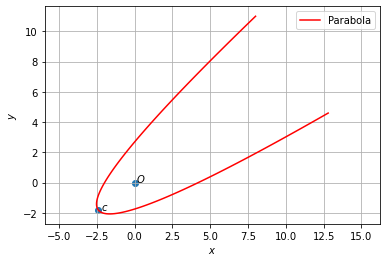
\includegraphics[width=\columnwidth]{assignment5parabola.png}
    \caption{Parabola with vertex c}
    \label{fig:fig1}
\end{figure}
\end{document}